\documentclass[a4paper,11pt]{article}

\usepackage[utf8]{inputenc} % Unicode support (Umlauts etc.)
\usepackage[ngerman]{babel} % Change hyphenation rules
\usepackage{ziffer} % , können in Zahlen verwendet werden ohne Formatierung kaputt zu machen
\usepackage[top=30mm,right=20mm,bottom=15mm,left=25mm,includefoot,headheight=32pt]{geometry} % Seitenränder

\usepackage{lmodern,textcomp} % The package supports the Text Companion fonts, which provide many text symbols (benötigt für €)
\usepackage[fleqn]{amsmath} % Formatierte Gleichungen
\usepackage{graphicx} % Grafiken
\usepackage{xcolor} % Farbe in Text
\usepackage{fancyhdr} % Seitenstil mit Kopfzeile etc.

\usepackage{cases} % Fallunterscheidungen mathematisch uebereinander

\usepackage{floatflt}

\pagestyle{fancy}
\fancyhf{}
\lhead{
    Lösung \\
    Übungsblatt 7
}
\rhead{Gruppe 3 \\Nils \textbf{Hodys}, Sascha \textbf{Majewsky}}
\rfoot{Seite \thepage}

\setlength{\parindent}{0cm} % Keine Einrückung der 1. Zeile eines Absatzes

\begin{document}

\raggedright % Alles Linksbündig

\section*{Aufgabe 1}

\subsection*{Entscheidungsvariablen}

\begin{align*}
& X_{EP} = ~\text{Palette mit 40 einfachen Platinen} \\
& X_{KP} = ~\text{Palette mit 40 komplexen Platinen} \\
 %
& Y_A = \left\{\begin{array}{l}
            1: ~\text{Standort A wird gebaut} \\
            0: ~\text{Standort A wird nicht gebaut} \\
          \end{array}\right. \\
%
&Y_B = \left\{\begin{array}{l}
            1: ~\text{Standort B wird gebaut} \\
            0: ~\text{Standort B wird nicht gebaut} \\
          \end{array}\right. \\
\end{align*}

\subsection*{Zielfunktion}
(Maximierung der hergestellten Platinen in Paletten zu je 40 Platinen) \\~\\

max. $z  = X_{EP} + X_{KP}$ \\

\subsection*{Kapazitätsrestriktionen Standort A}

\begin{align*}
X_{EP} + X_{KP} &\le ~ 73.125 + M_a(1-Y_a) && \big|~ \text{Max. Material schmelzen pro Woche} \\
X_{EP} + X_{KP} &\le ~ 48.875 + M_a(1-Y_a) && \big|~ \text{Max. Löten pro Woche} \\
X_{EP} + X_{KP} &\le ~ 66.500 + M_a(1-Y_a) && \big|~ \text{Max. Qualitätssicherung pro Woche} \\
0,31X_{EP} + 0,24X_{KP} &\le ~ 6500 + M_a(1-Y_a) && \big|~ \text{Verfügbarkeit Kupfer pro Woche} \\
0,12X_{EP} + 0,12X_{KP} &\le ~ 3900 + M_a(1-Y_a) && \big|~ \text{Verfügbarkeit Plastikplatinen pro Woche} \\
0,015X_{EP} + 0,025X_{KP} &\le ~ 2600 + M_a(1-Y_a) && \big|~ \text{Verfügbarkeit Wolfram pro Woche} \\
0,03X_{EP} + 0,02X_{KP} &\le ~ 5900 + M_a(1-Y_a) && \big|~ \text{Verfügbarkeit Stahl pro Woche} \\
0,055X_{KP} &\le ~ 550 + M_a(1-Y_a) && \big|~ \text{Verfügbarkeit Seltene Erden pro Woche} \\
\end{align*}

\subsection*{Kapazitätsrestriktionen Standort B}
\begin{align*}
X_{EP} + X_{KP} &\le ~ 95.625 + M_b(1-Y_b) && \big|~ \text{Max. Material schmelzen pro Woche} \\
X_{EP} + X_{KP} &\le ~ 60.375 + M_b(1-Y_b) && \big|~ \text{Max. Löten pro Woche} \\
X_{EP} + X_{KP} &\le ~ 85.500 + M_b(1-Y_b) && \big|~ \text{Max. Qualitätssicherung pro Woche} \\
0,31X_{EP} + 0,24X_{KP} &\le ~ 5700 + M_b(1-Y_b) && \big|~ \text{Verfügbarkeit Kupfer pro Woche} \\
0,12X_{EP} + 0,12X_{KP} &\le ~ 3200 + M_b(1-Y_b) && \big|~ \text{Verfügbarkeit Plastikplatinen pro Woche} \\
0,015X_{EP} + 0,025X_{KP} &\le ~ 1900 + M_b(1-Y_b) && \big|~ \text{Verfügbarkeit Wolfram pro Woche} \\
0,03X_{EP} + 0,02X_{KP} &\le ~ 5100 + M_b(1-Y_b) && \big|~ \text{Verfügbarkeit Stahl pro Woche} \\
0,055X_{KP} &\le ~ 410 + M_b(1-Y_b) && \big|~ \text{Verfügbarkeit Seltene Erden pro Woche} \\
\end{align*}


\subsection*{Weitere Restriktionen}
\begin{align*}
X_{EP} &\ge 1025 && \big|~ \text{Mindestanzahl Paletten einfacher Platinen} \\
X_{KP} &\ge 1025 && \big|~ \text{Mindestanzahl Paletten komplexer Platinen} \\
X_{EP}, X_{KP} &\ge 0 && \big|~ \text{NNB} \\
Y_a + Y_b &= 1 && \big|~ \text{Genau ein Standort} \\
Y_a , Y_b &\in \{ 1,0 \} && \big|~ \text{Binärvariablen} \\
\end{align*}


\section*{Aufgabe 2}

\subsection*{Entscheidungsvariablen}
$x_{d}$: Produktionsmenge Fahrrad Deluxe in Stück pro Woche \\
$x_{n}$: Produktionsmenge Fahrrad Normal in Stück pro Woche \\


\subsection*{Bestimmung der Optima}
Bestimmung $z_{1}^{\text{Opt}} = 78000$ via Solver \\
Bestimmung $z_{2}^{\text{Opt}} = 7000$ via Solver \\~\\

\subsubsection*{Umformung}
\begin{align*}
\text{min } z_{2} &= 30x_{d} +20x_{n} \\
\Rightarrow \text{max } z_{2}^{'} &= -30x_{d} -20x_{n} \\
\end{align*}
Daher gilt auch $z_{2}^{'\text{Opt}} = -7000$ \\

\vspace{4mm}

\subsubsection*{Solverlösungen}
(Bestimmung der Optimalen Teilfunktionswerte) \\~\\

\begin{minipage}{1\textwidth}
  \centering
  \begin{minipage}{.5\textwidth}
    \centering
    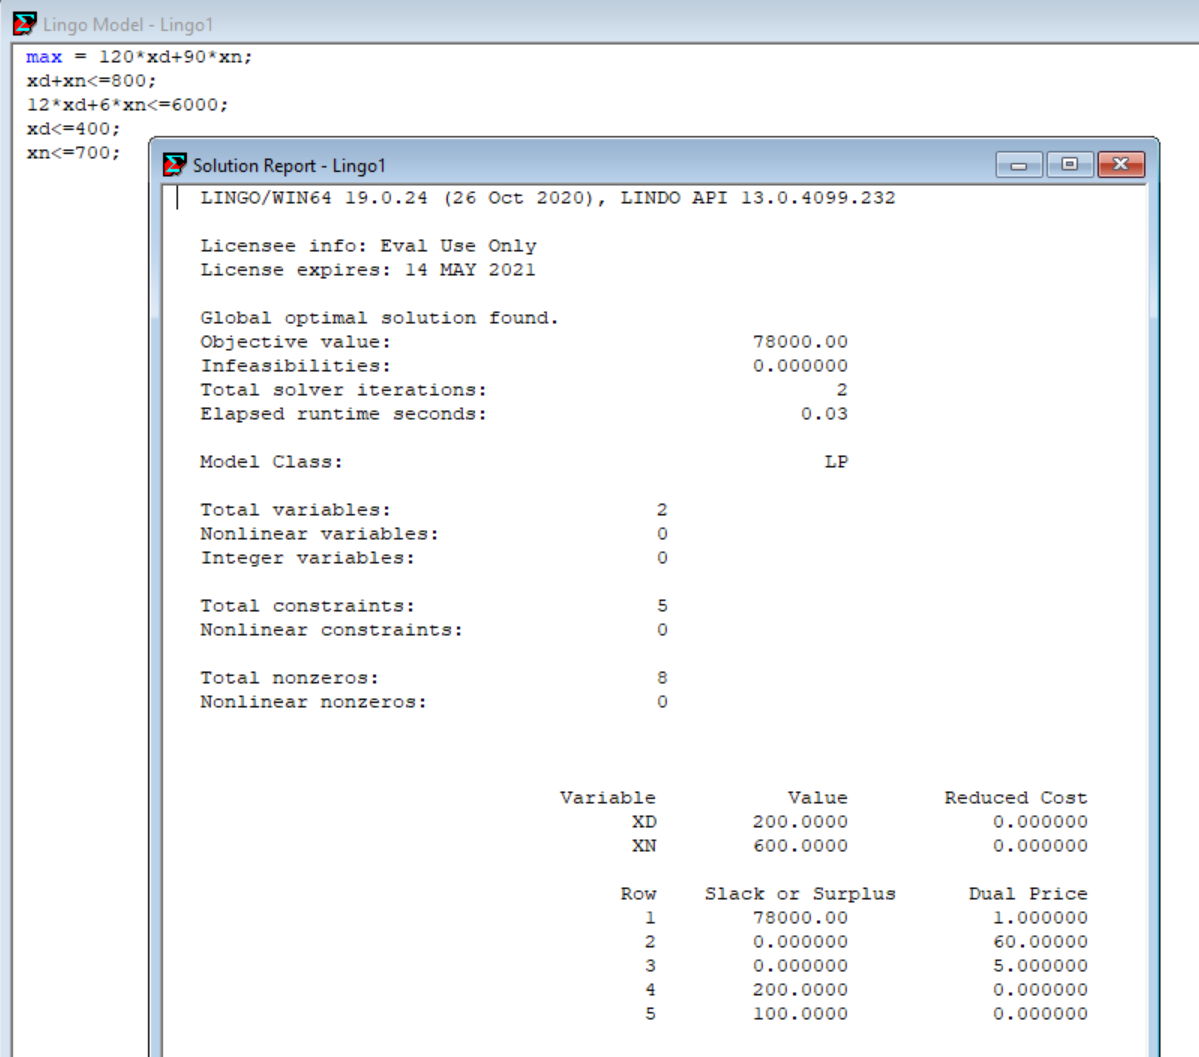
\includegraphics[width=1\linewidth]{src/blatt_7_aufgabe_2_solverloesung_1.png}
  \end{minipage}%
  \begin{minipage}{.5\textwidth}
    \centering
    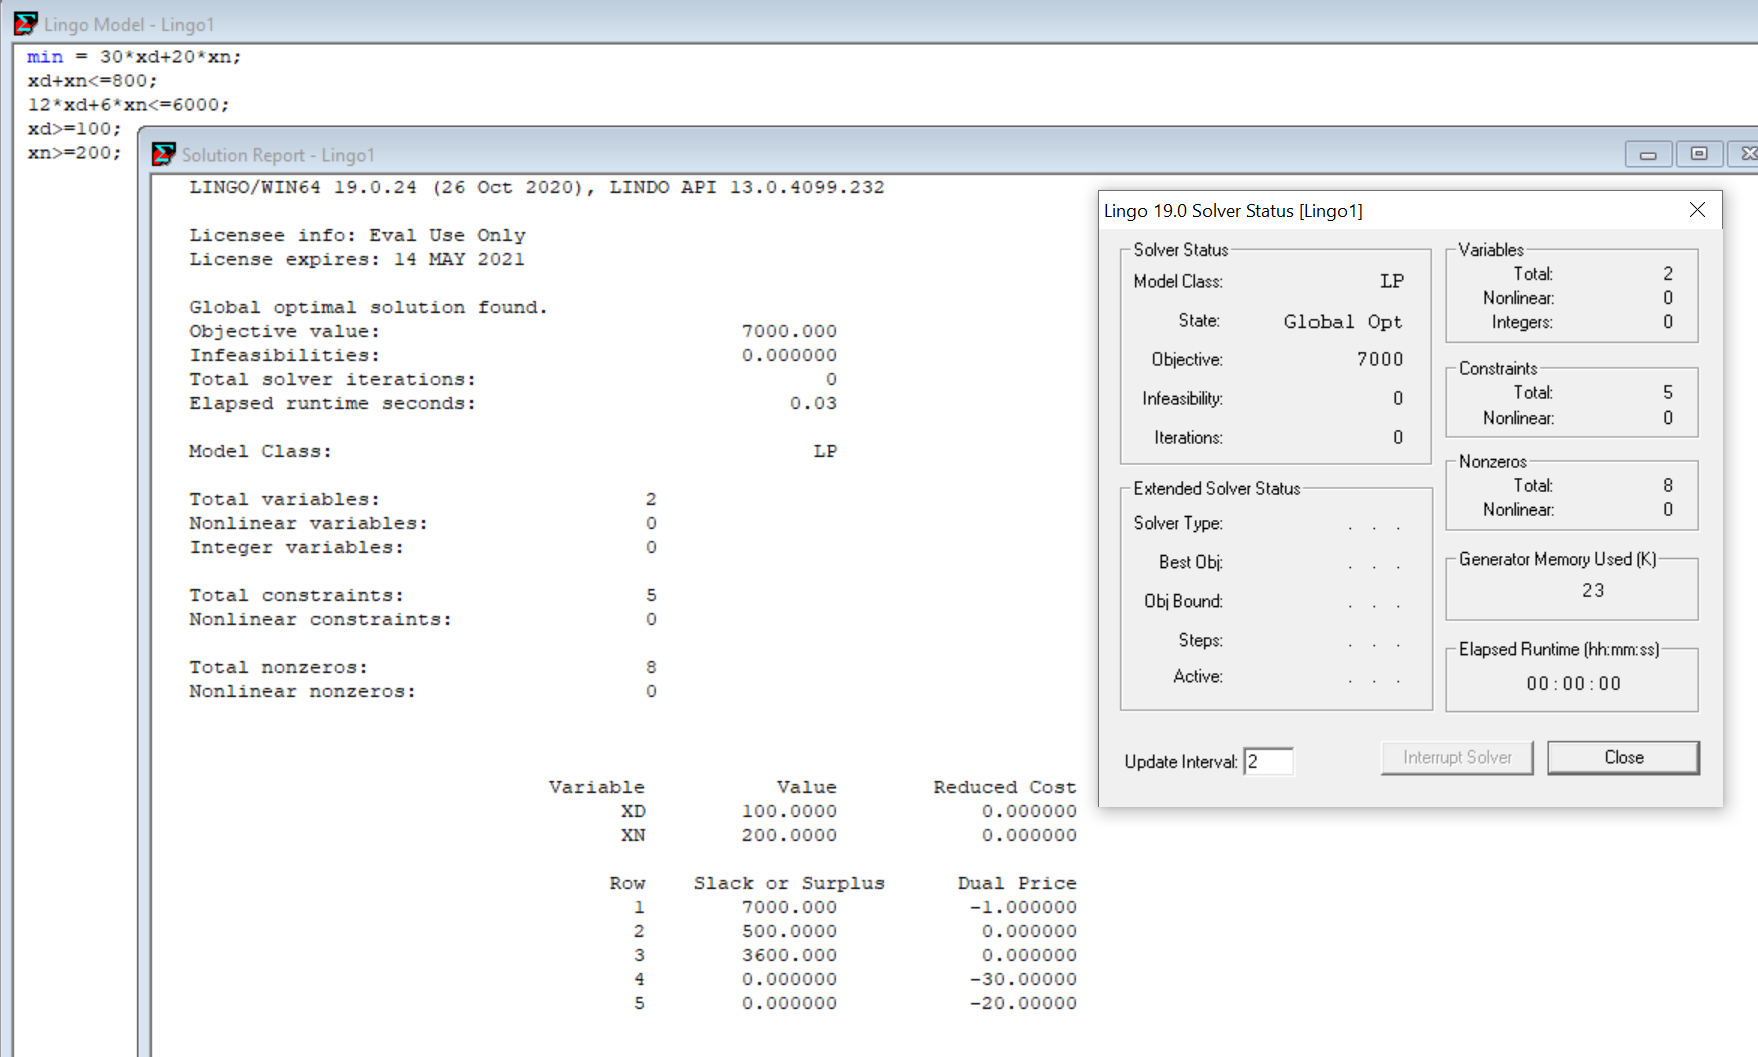
\includegraphics[width=1\linewidth]{src/blatt_7_aufgabe_2_solverloesung_2.png}
  \end{minipage}
\end{minipage}


\subsection*{LP-Modell}

\begin{align*}
    \text{min } &z \\~\\
    \text{s.t. } & x_{d} + x_{n} \le 800 && \big|~ \text{Max. Produktionsmenge} \\
    & 12x_{d} + 6x_{n} \le 6000 && \big|~ \text{Max. verfügbare Zeit} \\
    & -30x_{d} -20x_{n} + v_{1} = -7000 && \big|~ \text{Einsetzen $z_{2}^{'}$ mit $z_{2}^{'Opt}$ } \\
    & 120x_{d} + 90x_{n} + v_{2} = 78000 && \big|~ \text{Einsetzen $z_{1}$ mit $z_{1}^{Opt}$ } \\
    & x_{d} \le 400 && \big|~ \text{Max Anzahl Deluxe pro Woche} \\
    & x_{n} \le 700 && \big|~ \text{Max Anzahl Normal pro Woche} \\
    & x_{d} \ge 100 && \big|~ \text{Min Anzahl Deluxe pro Woche} \\
    & x_{n} \ge 200 && \big|~ \text{Min Anzahl Normal pro Woche} \\
    & v_{1} \le z &&  \text{} \\
    & v_{2} \le z && \text{} \\
    & x_{d}, x_{n}, v_1, v_2 \ge 0 && \big|~ \text{NNB} \\
\end{align*}

\subsubsection*{Solverlösung}

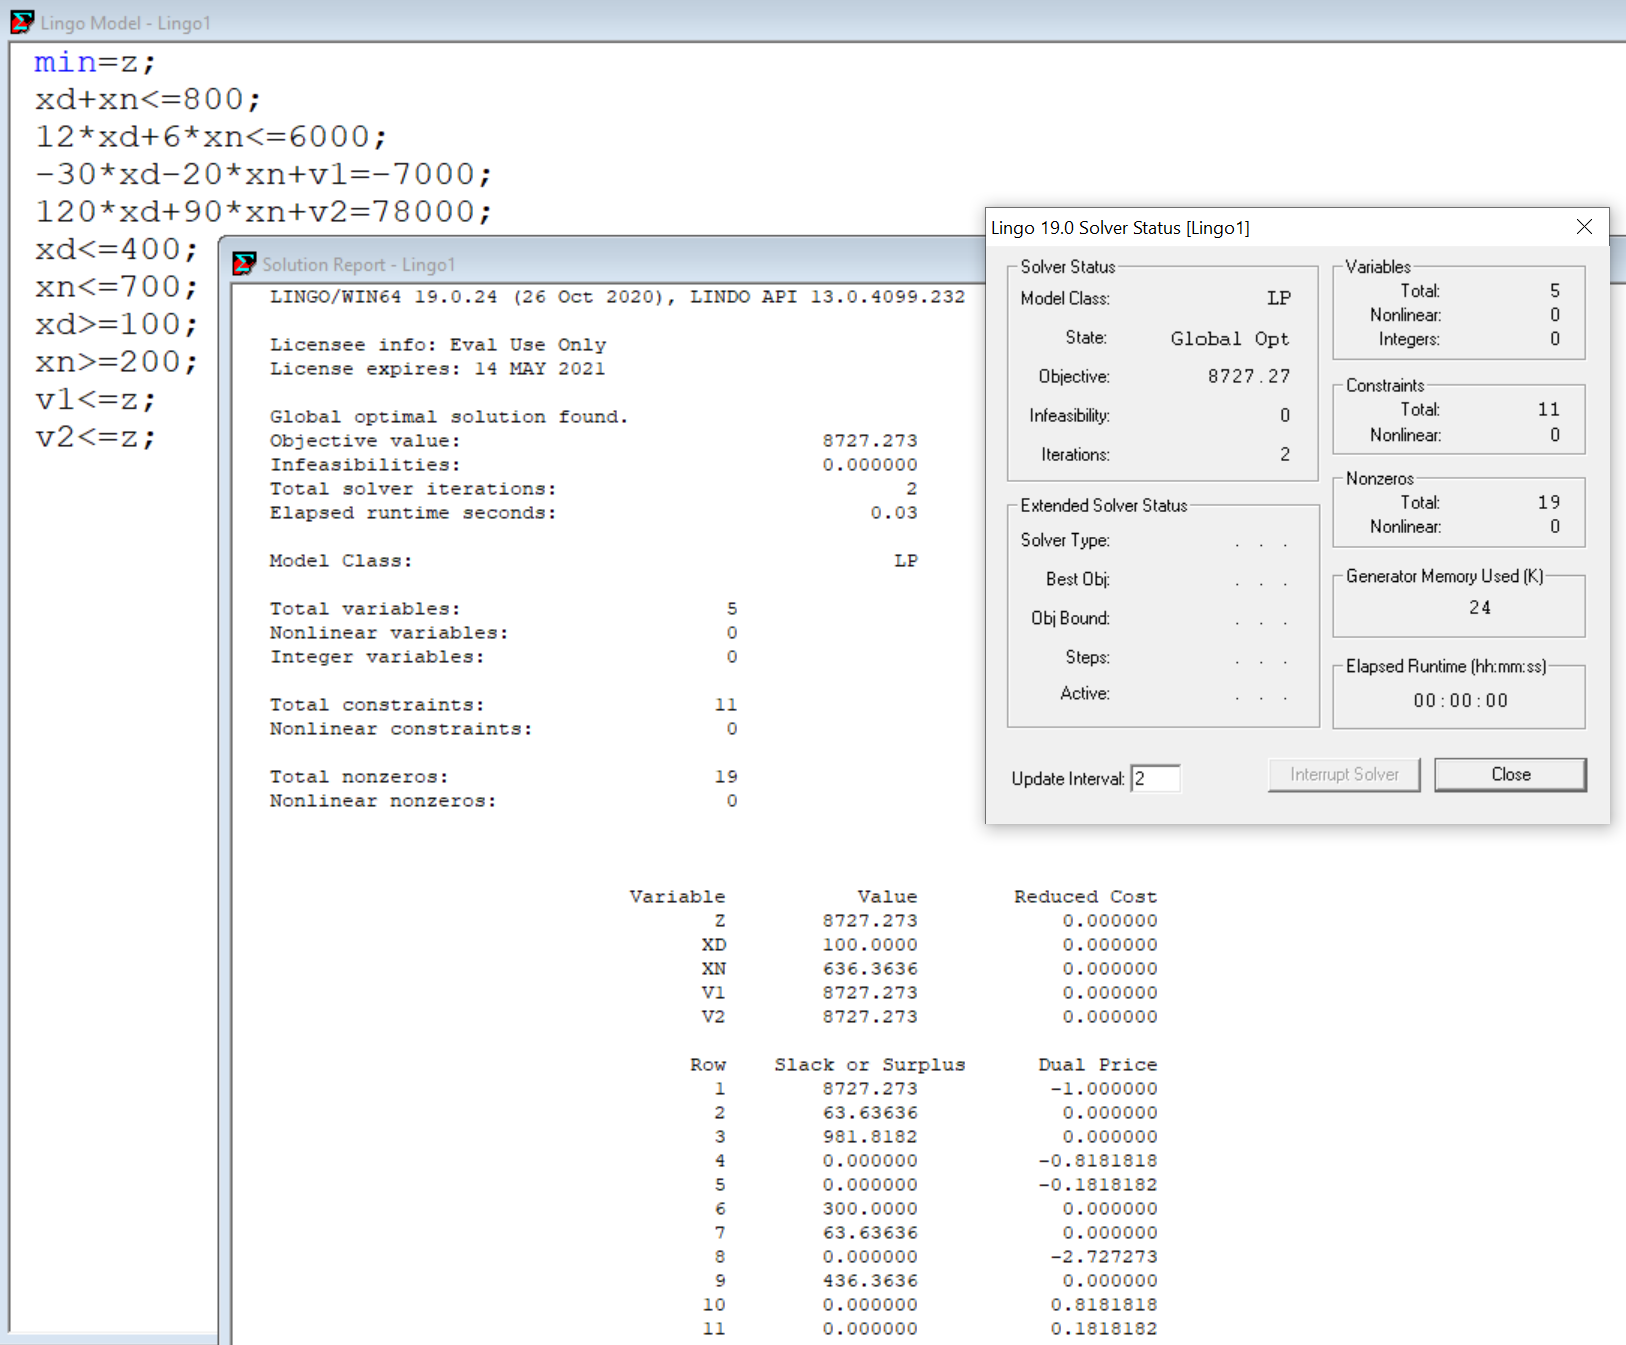
\includegraphics[width=1\linewidth]{src/blatt_7_aufgabe_2_solverloesung_3.png}

\end{document}